\section{Introduction}\label{sec:introduction}
% no \IEEEPARstart

Animals use their tails in a variety of ways: to propel through water; to help improve locomotion and balance; and some, like for instance monkeys, have prehensile tails that allow them to grasp trees. Balance control while running and hopping, even glide control and climbing are some examples of how a tail is helping animals by providing robust locomotion \cite{Thomas:Nature2012}. The use of a tail, or inertial appendages in general, for dynamic stabilization has been reported in dinosaurs, lizards, cats, primates and even humans \cite{ostrom1969osteology,PijnappelsSringer,Walker199841,JusufiIOP2010}. One of the challenging tasks in biologically inspired robotics is to extract the knowledge from and not simply mimic the nature. Therefore, we seek nature-like solutions on how to use additional appendages to help robot locomotion in the similar way as an animal would do.  

A tail can balance the robot’s body in both static and dynamic sense. The main technique of using a tail as a dynamic stabilizer for quadruped robot locomotion is to apply additional forces/torques on its body. Uniroo \cite{zeglin1991uniroo} is one of the first robots which use single degree of freedom active tail to maintain constant body pitch with the purpose of emulating a hopping kangaroo. A lizard-inspired active tail stabilization presented in \cite{conf/iros/Chang-SiuLTF11} uses a tail on a wheeled car, thus providing a robust maneuvering over difficult terrain. The basic principal of the conservation of momentum for pitch control stability only. The MIT Cheetah robot \cite{DBLP:conf/iros/BriggsLHK12} uses a tail to improve robots running capabilities and perform up to 30mph runs. Additionally, the authors analyze several other artificial mechanisms which can be used to apply non-contact forces/torques like: reaction wheel, reaction mass, thrusters etc. In \cite{PullinICRA12}, Pullin et all compared the use of a tail to classical differential drive steering for different surface conditions on a crawling mobile robot OctoRoACH. They showed how a tail could be used when rapid turning or evasive maneuvers are required as well as on low friction surface conditions. Learning from Air robots, one can apply the techniques used in \cite{Korpela2013ICRA,Orsag2012JINT} to model the dynamics of inertial appendages and the effect they have on the underlying robot body. This paper however, wishes to address an alternative use for a tail, its static balancing capabilities. We envision a tail as a counterweight, capable of shifting its center of mass so as to balance the body of the robot.

\begin{figure}
	\centering
	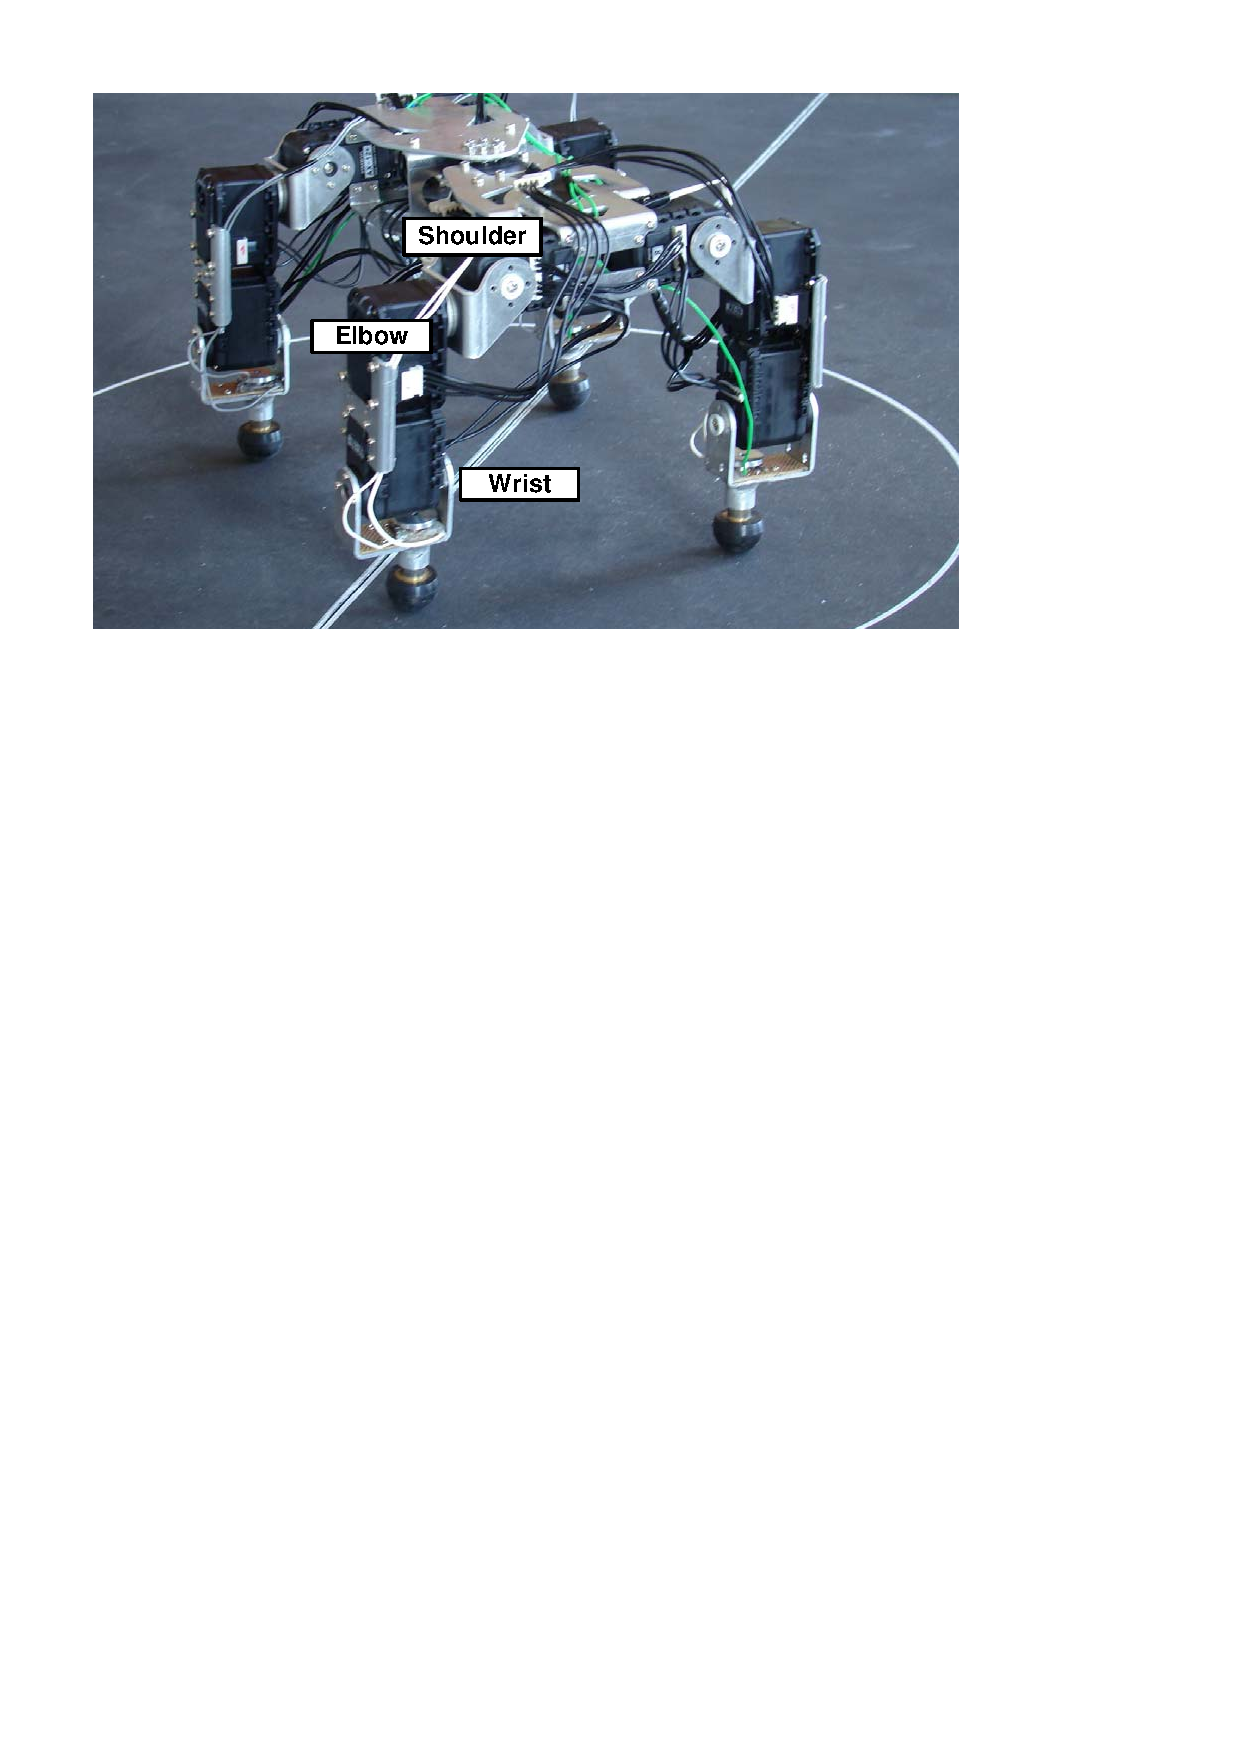
\includegraphics[width=85mm]{./pictures/Dynarobin_introduction_image.pdf}
	\caption{Dynarobin}
	\label{fig:Dynarobin}
\end{figure}

Inspired by the agility of human and animal locomotion, over the last few decades  the number of research groups presented numerous robot leg designs, and the associated modeling and control \cite{CambridgeJournals:1345088}. The predominant method for the modeling of quadruped locomotion gaits like walking, running, trotting, and bouncing is a spring-mass model\cite{Blickhan01}. This paper postulates that a single leg, hopping locomotion can also be described with a spring-mass model. In order to obtain a compliant robot leg behavior, impedance control is used to emulate a virtual spring-mass system \cite{Havoutis01}. Connecting four legs with one central body complex dynamic problems arises. In order to provide a stabile quadruped hopping sequence a lot of parameters needs to be observed: mass distribution, active and passive leg stiffness, ground stiffness, etc. This paper investigates how to improve locomotion stability of a dynamical system of four spring-masses by using the tail-like inertial appendage. 

In section \ref{sec:MathModel} a mathematical model of quadruped robot Dynarobin (Fig. \ref{fig:Dynarobin}) together with kinematic and dynamic model of the tail is introduced. A single leg dynamics is modeled to mimic the behavior of an active spring-mass system. Building upon the results from \ref{sec:MathModel}, a recursive balancing algorithm is introduced in \ref{sec:Algorithm}. The algorithm is tested in the simulation environment which is described in section \ref{sec:simulation}, along with the simulation results. 





% Some research uses advanced variable stiffnes leg design %\cite{Hurst_2004_4785}\cite{Galloway}\cite{Jun:2009:DSV:1703775.1704089} which allows robot to run over a large variety %of terrains while adjusting their leg stiffness. All this research suggests that quadrupedal robot can be dynamically 5modeled as mass supported on four spring legs as shown in fig. 


